\documentclass[11pt]{article}
\usepackage{bookmark}
\usepackage{algorithm}
\usepackage{algpseudocode}
\usepackage{amsfonts}
\usepackage{amsmath}
\usepackage{amssymb}
\usepackage{amsthm}
\usepackage{bm}
\usepackage{color}
\usepackage{comment}
\usepackage{float}
\usepackage{graphicx}
%\usepackage[hidelinks]{hyperref}
\usepackage{makecell}
\usepackage[caption=false,font=footnotesize,subrefformat=parens,labelformat=parens]{subfig}
\usepackage{wrapfig}
\usepackage{url}
\usepackage[table]{xcolor}
%
\setlength{\parindent}{0.25in}
\setlength{\parskip}{.05in}
\pagestyle{plain}
%Title, date an author of the document
\title{Progress Report}
\author{Bardia Mojra}


\begin{document}
\maketitle
\thispagestyle{empty}

\bigskip
\bigskip
\begin{center}
      Robotic Vision Lab
\end{center}

\begin{center}
      The University of Texas at Arlington
\end{center}

\newpage

\section{Specific Research Goals}
\begin{itemize}
      \item VPQEKF: Write and submit paper by September 14th (ICRA)
      \item AFRL Proposal:
      \item NBV-Grasping.
      \item Universal pose estimation or a novel and superior approach.
\end{itemize}

\section{To Do}
\begin{itemize}
  \item Catch up on my reading list.
  \item PVQEKF:
  \begin{itemize}
      \item Keep improving and debugging the QEKF code.
      \item Develop object tracking and robust-to-truncation feature.
      \item Get ROS environment up and running. -- Next: test header include bug theory.
  \end{itemize}
  \item AFRL: Controls and DNN research.
  \item Real-time pose estimation demo.
  \item NBV-Grasping:
      \begin{itemize}
      \item Update URDF and Xacro files for UR5e to include sensor, sensor mount (with offset), and the gripper. -- Next
      \item Add movement constraints for tables and scenes.
      \item Write two IK functions for gripper and sensor, one for each. It should plug-in with MoveIt configurator.
      \item Research and implement point-cloud data to training TensorFlow models.
      \item Learn and implement GraspIt package.
      \end{itemize}
  \item MSI Fellowship: On pause.
\end{itemize}

\section{Reading List}
\begin{itemize}
      \item Vision-based robotic grasping from object localization, object pose estimation to grasp estimation for parallel grippers - a review \cite{du2020vision} - On-going.
      \item Leveraging feature uncertainty in the pnp problem \cite{ferraz2014leveraging}.
      \item Normalized objects \cite{Wang_2019_CVPR}.
      \item Berk Calli's YCB \cite{calli2015ycb}.
      \item NASA papers \cite{NASATech44:online}.
      \item Roadmap \cite{roadmap251:online}.
\end{itemize}

\section{Progress}
The following items are listed in the order of priority:
\begin{itemize}
      \item VPQEKF: This week, I mostly worked on the QEKF project and I am still getting
      inconsistent results. Figure 1, shows measurements vs. estimated translation where estimation moves in the opposite direction. Figure 2 shows translation measured and estimated values for the first 15 steps and it appears and it turns early on in the navigation process.
      Figure 3 shows full state measurements vs. estimations for QEKF.

      \begin{figure}
            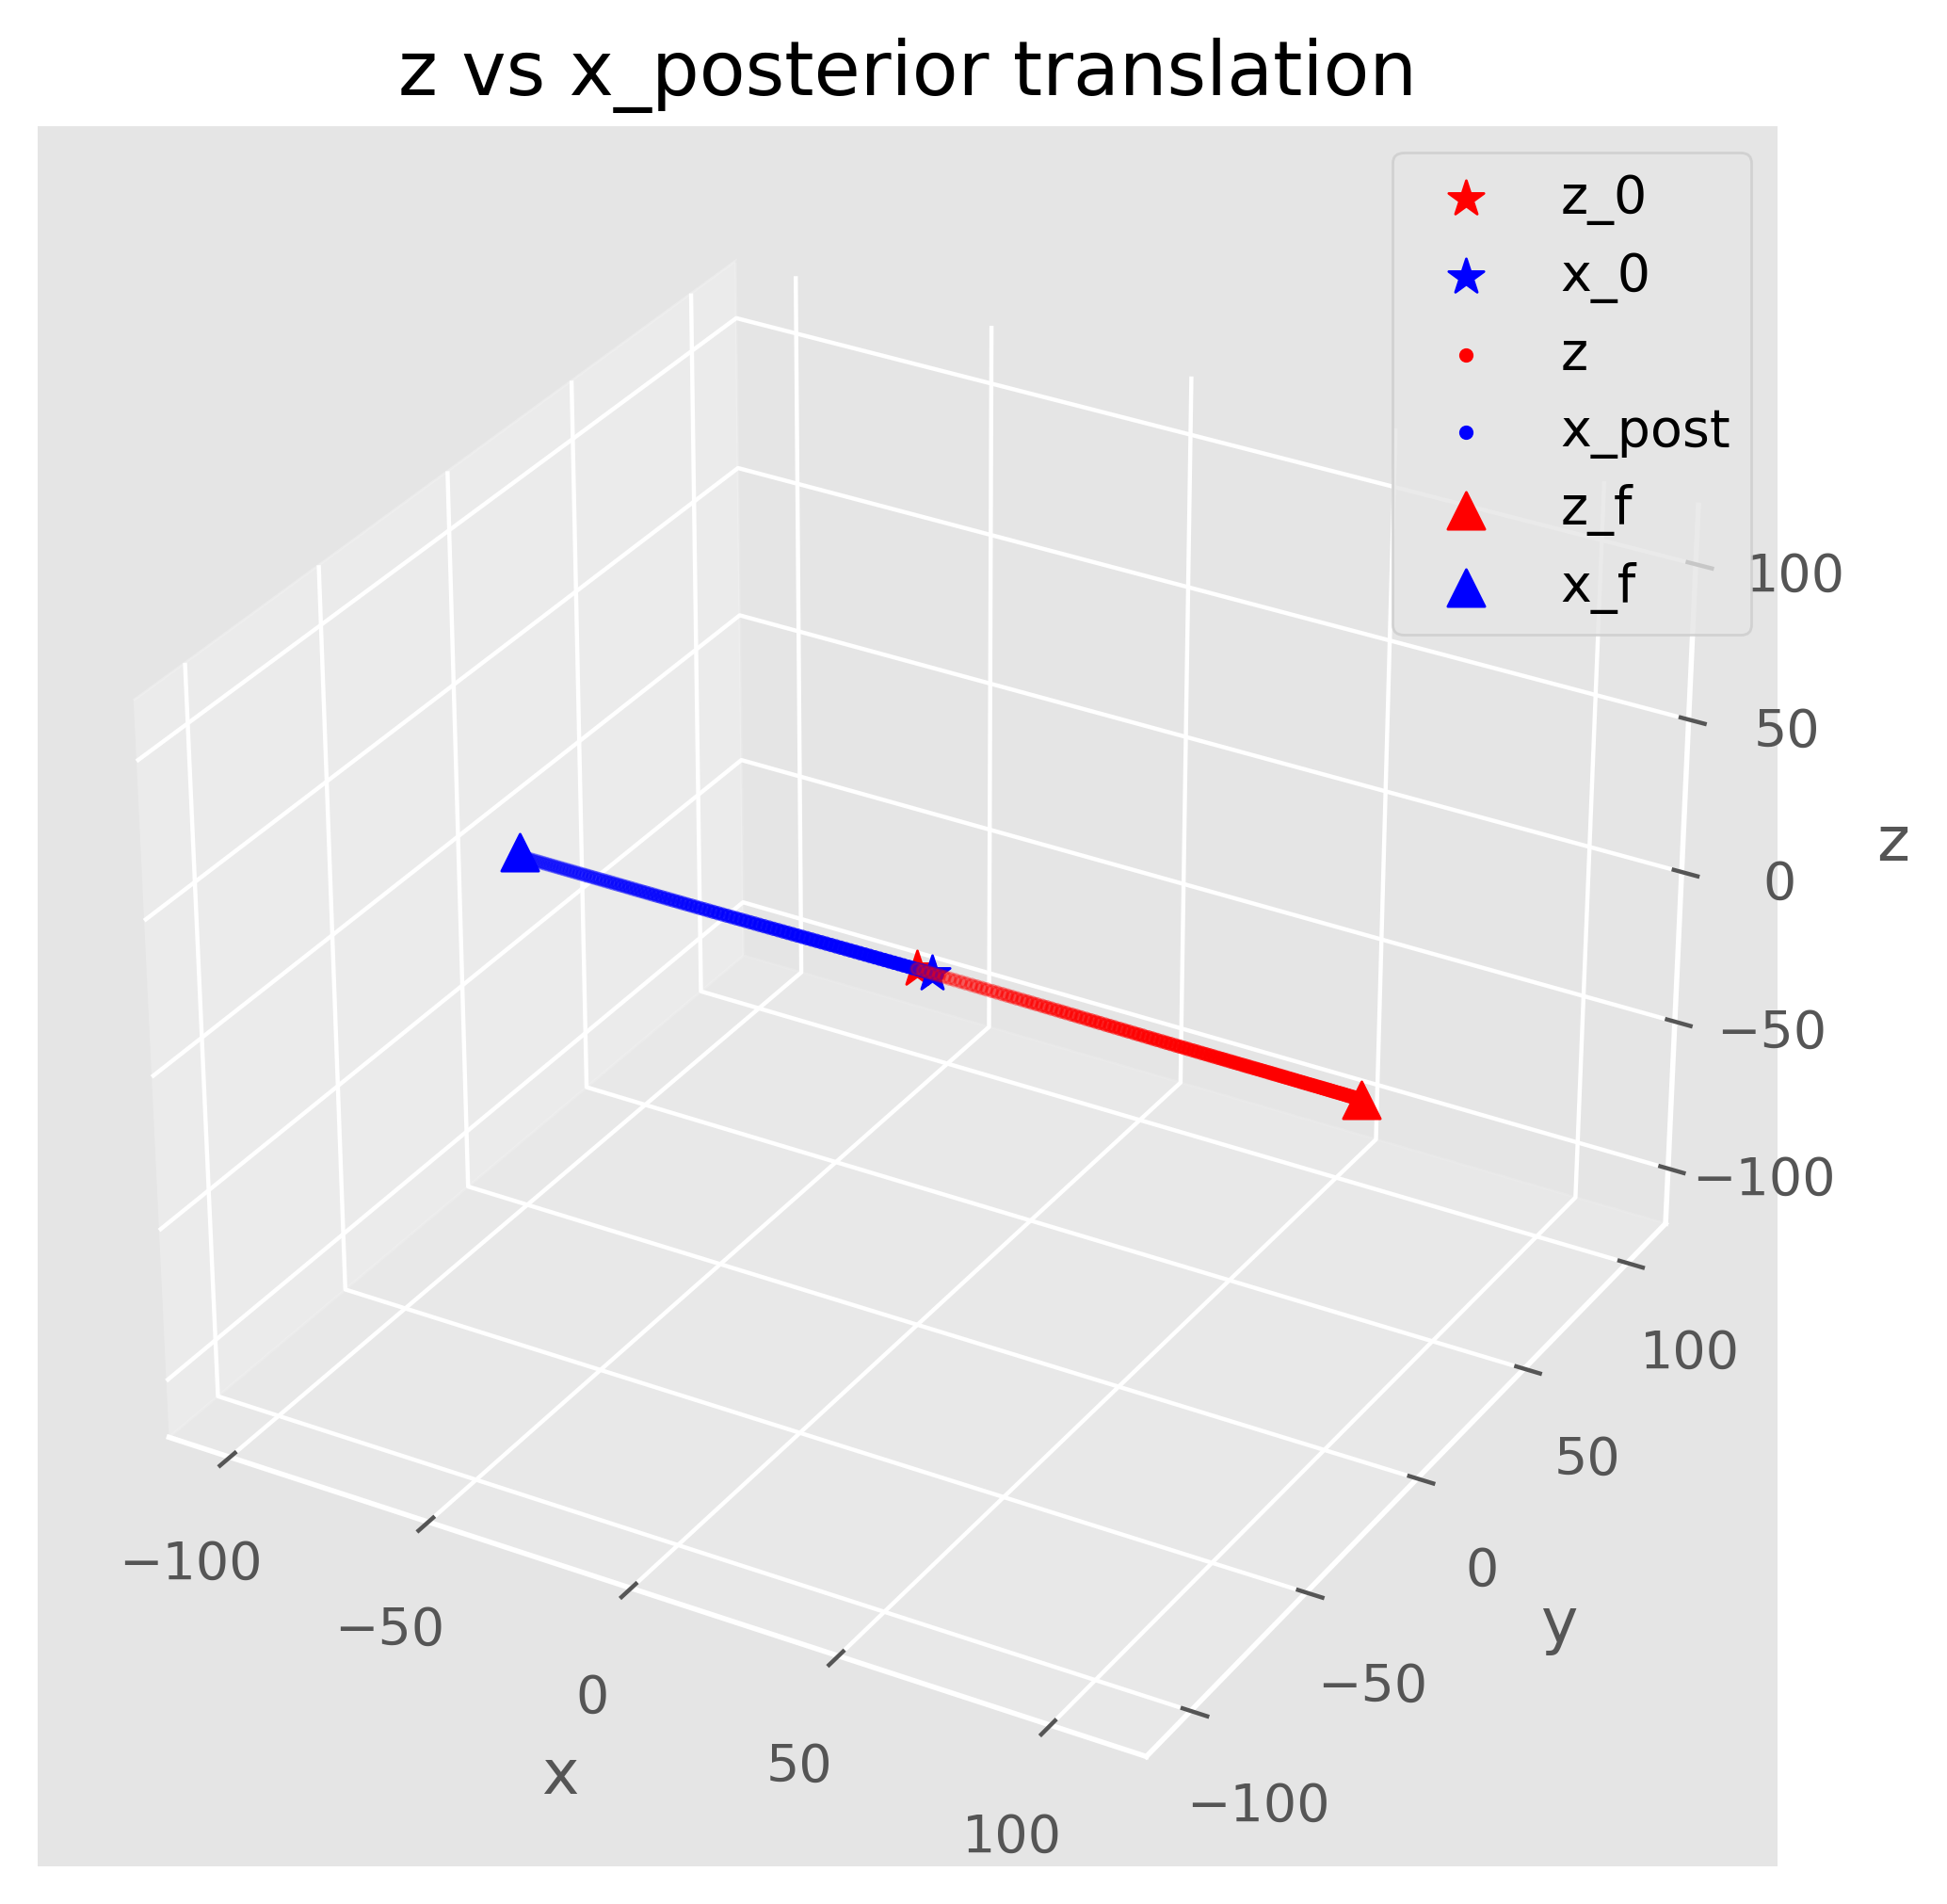
\includegraphics[width=\linewidth]{fig01.png}
            \caption{KITTI 001 - Measurement vs Posterior Est. Translation.}
            \label{fig:meas_vs_post}
      \end{figure}

      \begin{figure}
            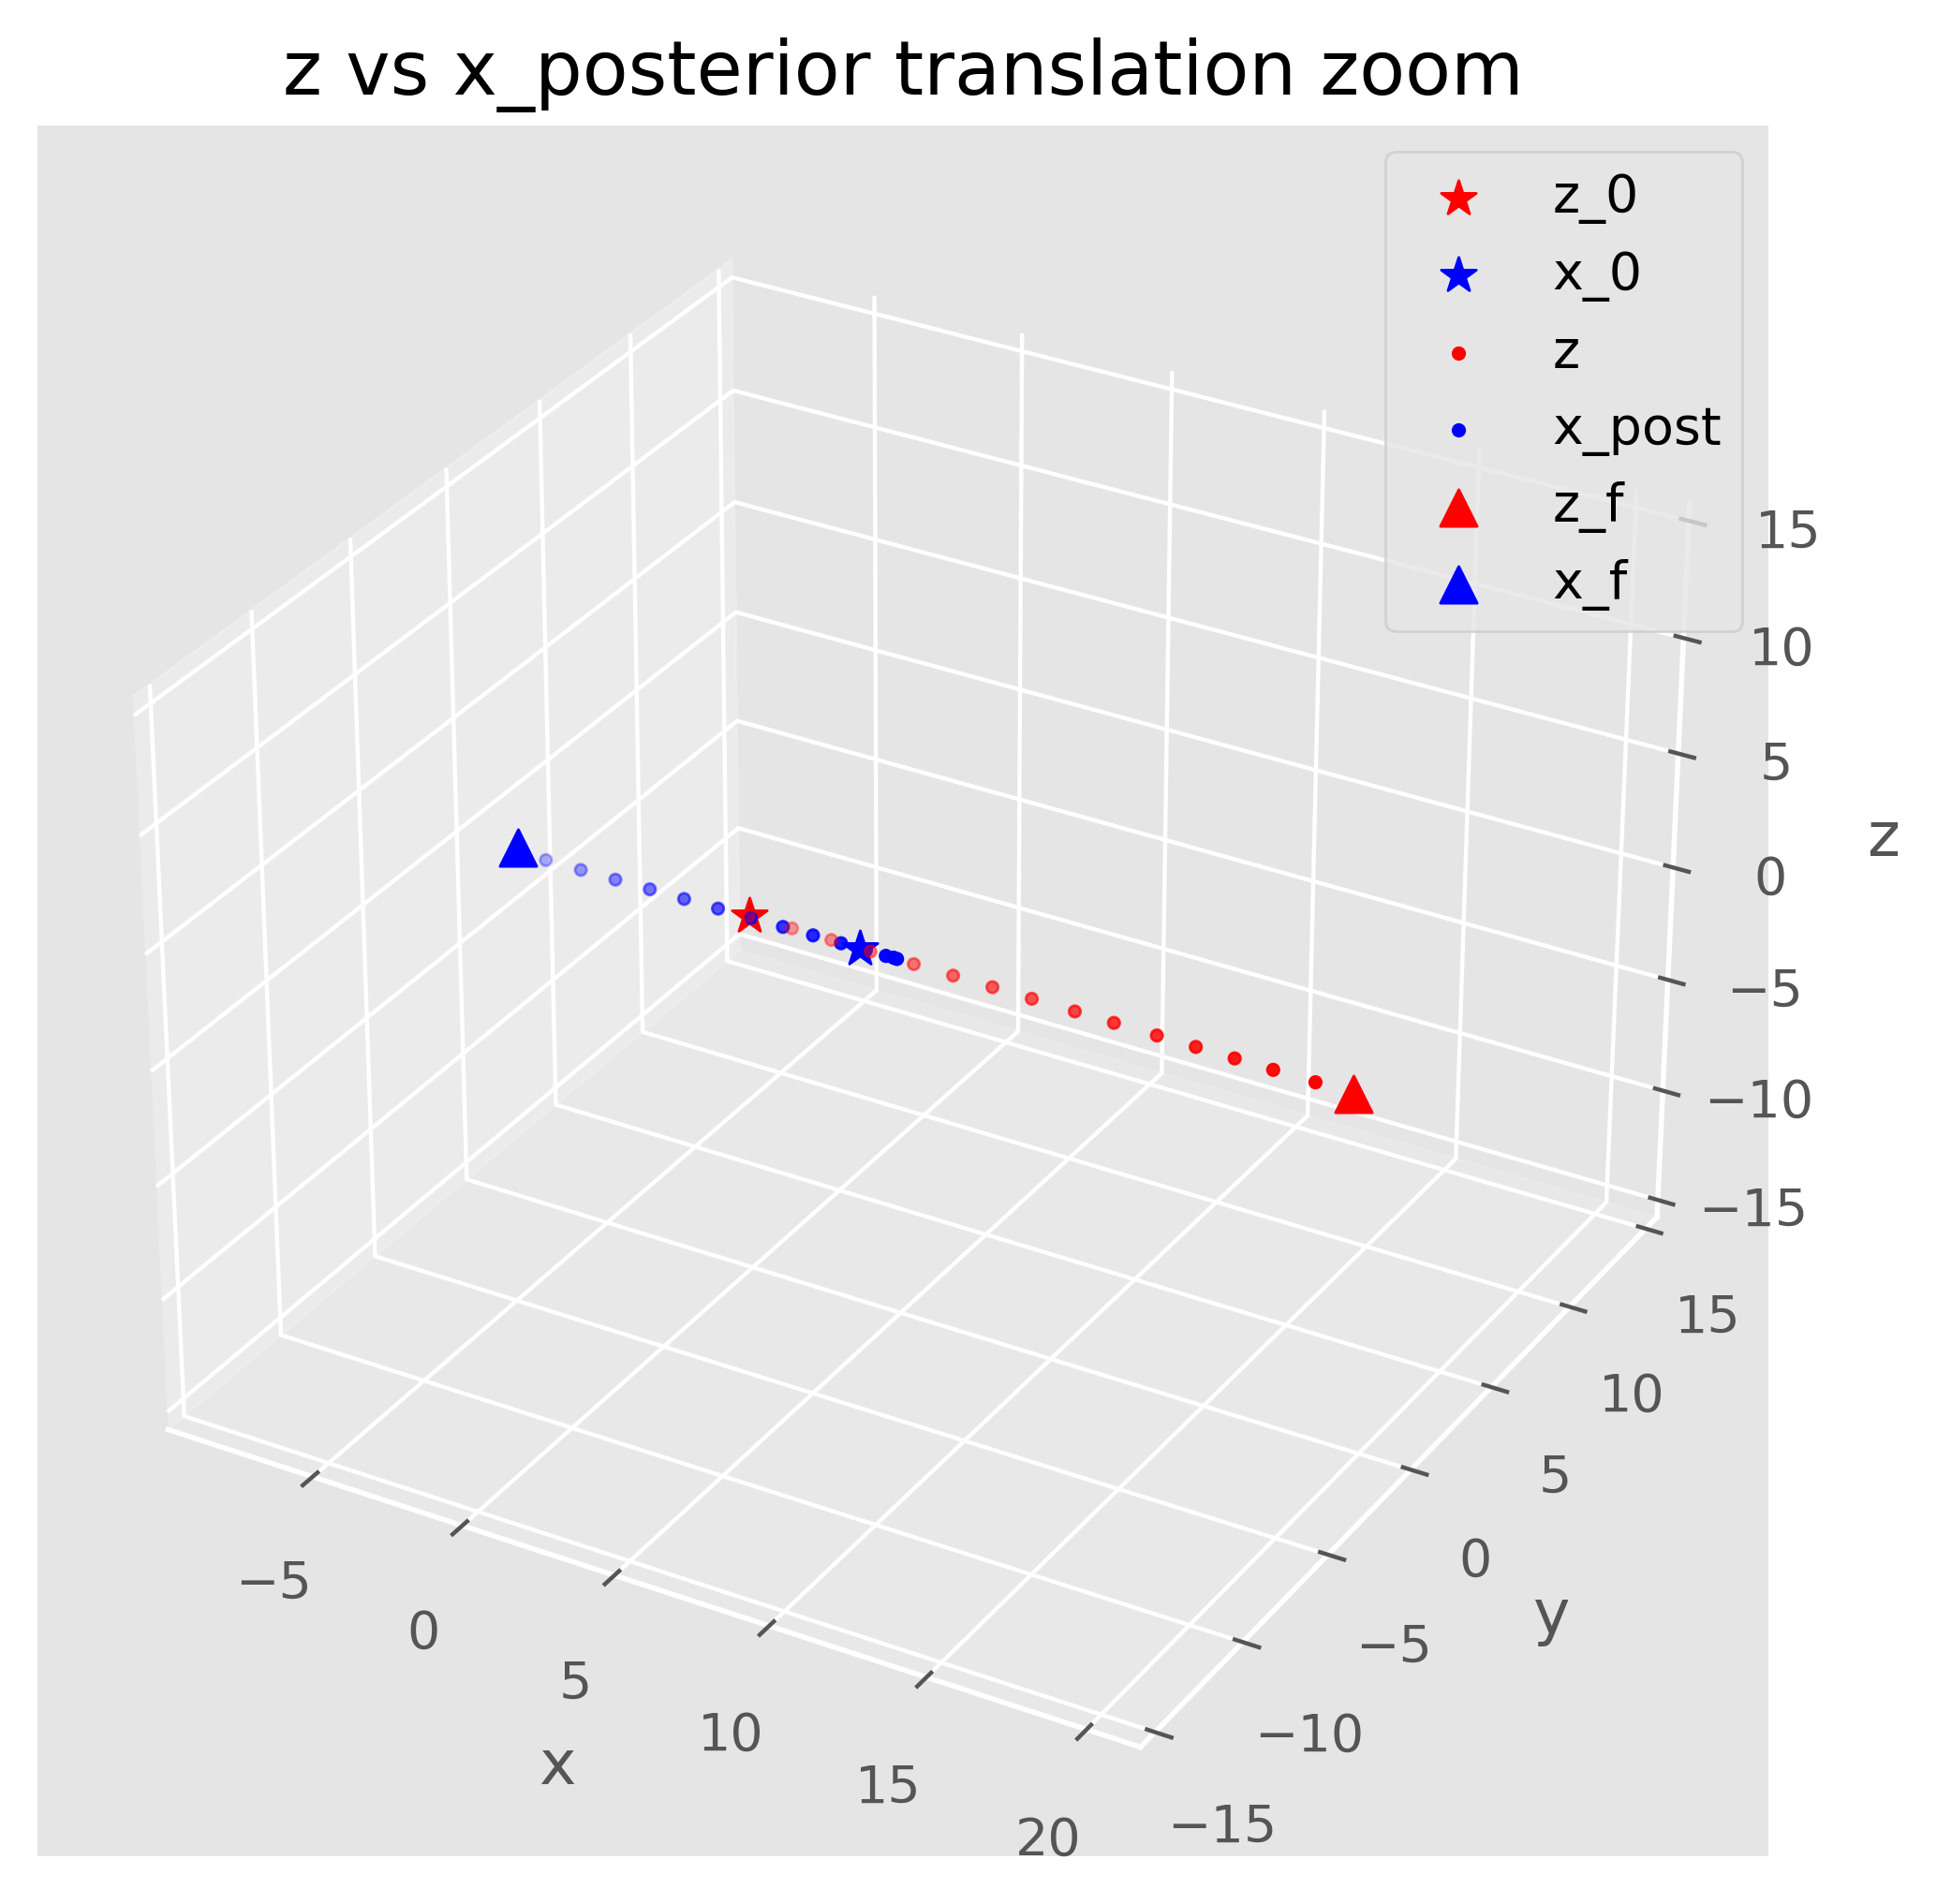
\includegraphics[width=\linewidth]{fig02.png}
            \caption{KITTI 001 - Measurement vs Posterior Est. Translation Zoom.}
            \label{fig:meas_vs_post_zoom}
      \end{figure}

      \begin{figure}
            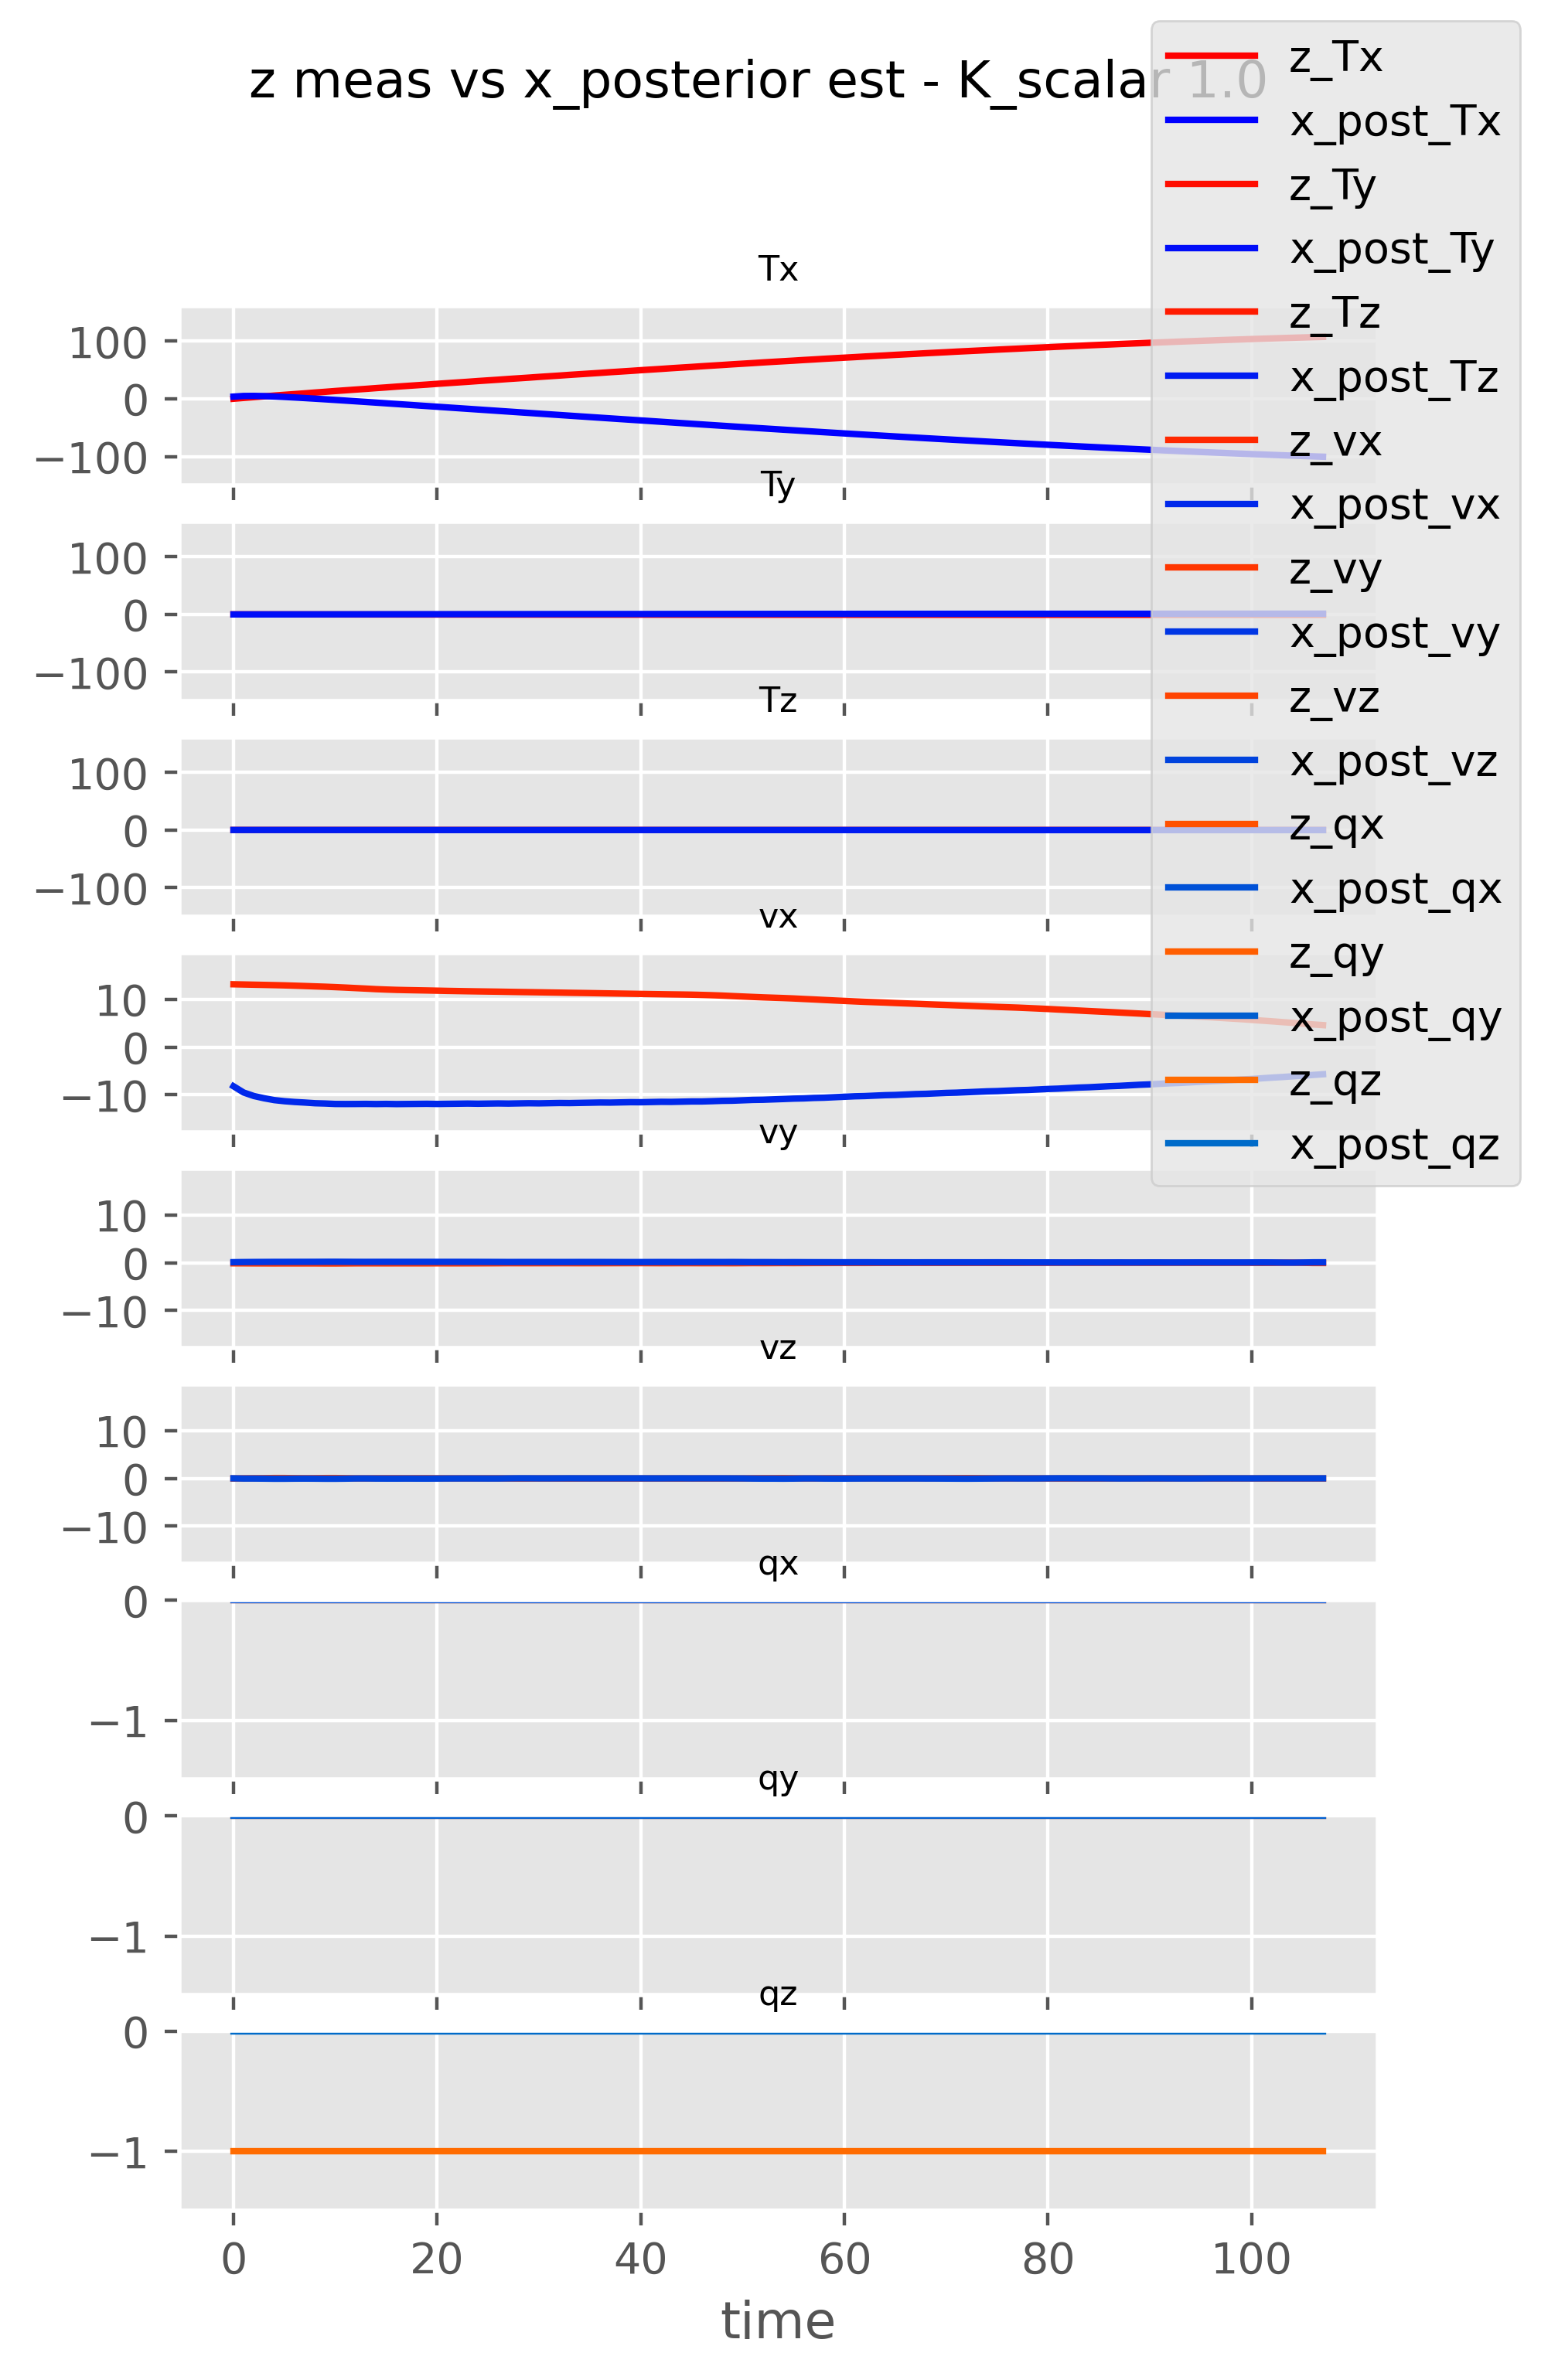
\includegraphics[width=\linewidth]{fig03.png}
            \caption{KITTI 001 - Measurement (\textit{z}) vs Posterior Estimate (\textit{x-post}).}
            \label{fig:meas_vs_post_iso}
      \end{figure}


      Figure \ref{fig:meas_vs_post} shows translation measurement (\textit{z}) vs estimate (\textit{x-post}) translation in 3D.
      Figure \ref{fig:meas_vs_post_zoom} shows translation measurement (\textit{z}) vs estimate (\textit{x-post}) in 3D for the first 15 samples.
      Figure \ref{fig:meas_vs_post_iso} shows all measurements vs estimations.

      \item AFRL: I think I would be most excited about combining controls and DNN methods for perception, odometry, navigation or manufacturing applications.

      \item NBV Grasping Project: No update.
      \item NASA MSI Fellowship: Need to read more NASA papers. -- On pause.
      \item PyTorch Tutorials: Transfer learning.
      \item Pose Estimation: On pause.
      \item SD Team: No update.
      \item EE Autonobots: No update.
\end{itemize}

%\newpage

\section{Immediate Plans - Summer 2021:}
The following items are listed in the order of priority:

\begin{itemize}
      \item UTARI: Dr. Gans' pose and velocity estimation paper.
      \item NBV-Grasping:
      \item Pose estimation: Survey paper.
\end{itemize}

\section{Intermediate Goals - Fall 2021:}
\begin{itemize}
      \item Pose estimation: I must be finished with implementation, perhaps make some improvements, and should be working on a paper for ICRA or CVPR.
      \item Scene understanding and active learning: After pose estimation, I want to expand my research into scene understanding and active learning in the context of advanced manufacturing.
      \item ARIAC: Once I am up to speed, I will do the ARIAC workshops/tutorials and will talk to Jerry about possible contributions.
\end{itemize}


%Sets the bibliography style to UNSRT and import the
\newpage
\bibliography{ref}
\bibliographystyle{ieeetr}

\end{document}
